\documentclass[12pt]{article}
\usepackage{float, amsmath, amssymb, amsthm, algorithm, algorithmic, graphicx, caption, subcaption, mathrsfs, color, cancel, verbatim, cite, authblk, mathtools}
\usepackage{enumitem}

\def\upint{\mathchoice%
    {\mkern13mu\overline{\vphantom{\intop}\mkern7mu}\mkern-20mu}%
    {\mkern7mu\overline{\vphantom{\intop}\mkern7mu}\mkern-14mu}%
    {\mkern7mu\overline{\vphantom{\intop}\mkern7mu}\mkern-14mu}%
    {\mkern7mu\overline{\vphantom{\intop}\mkern7mu}\mkern-14mu}%
  \int}
\def\lowint{\mkern3mu\underline{\vphantom{\intop}\mkern7mu}\mkern-10mu\int}

\let\oldemptyset\emptyset
\let\emptyset\varnothing

\setlength{\oddsidemargin}{0in}
\setlength{\evensidemargin}{\oddsidemargin}
\setlength{\textwidth}{6.5in}
\setlength{\topmargin}{-.25in}
\setlength{\headheight}{0in}
\setlength{\headsep}{0in}
\setlength{\topskip}{0in}
\setlength{\textheight}{9.5in}
\font\bigbf = cmbx10 scaled \magstep1
\font\medbf = cmbx10 scaled \magstephalf
\font\medrm = cmr10 scaled \magstephalf
\font\bigrm = cmr10 scaled \magstep1

\usepackage[english]{babel}
\usepackage[utf8]{inputenc}
\usepackage[colorinlistoftodos]{todonotes}

\title{Harmonic Analysis}
\begin{document}
\noindent \textbf{Oscillations in Harmonic Analysis} \\
\noindent July 2nd, 2018 \\
\noindent \textbf{Lecture 1: Eyvindur Palsson} \\
\noindent www.math.vt.edu/people/palsson/pcmi.html \\

\noindent \textbf{General Overview of Harmonic Analysis} \\
Harmonic analysis (HA), as with many subjects in mathematics, is closely related to other subjects in mathematics. In particular, it has great connections with Partial Differential Equations (PDE), Number Theory (NT), Geometric Measure Theory (GMT), and Combinatorics (C). Harmonic analysis can be used as a tool to solve problems in these related subjects, and vice-versa. \\

\begin{figure}[H]
\centering
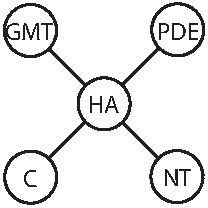
\includegraphics[width=0.25\textwidth]{1Overview.pdf}
\caption{}
\end{figure}

\noindent \textbf{Combinatorics} \\
Suppose that I want to select $k$ objects from a set of $n$ objects. For my first choice, I have $n$ different choices. For my second choice, I have $n-1$ different choices (since I cannot choose the first object again). If we repeat this pattern, we find that there is 
$$n(n-1)(n-2) \cdots (n-k+1)$$
possible ways that we can choose $k$ objects. However, we don't care in which order we choose these objects. If I select $A$, then $B$, it shouldn't be any different that if I select $B$, then $A$. Therefore, we remove these repetitions by dividing by the number of ways to rearrange our list of selections. This yields the following formula:
$$\frac{n(n-1)(n-2) \cdots (n-k+1)}{k(k-1)(k-2)\cdots 1}$$
\noindent We denote this formula using the following notations: \\
$$ \binom{N}{2} = \frac{n!}{k!(n-k)!} = \frac{n(n-1) \cdots (n-k+1)}{k(k-1)\cdots 1}$$
\noindent One important problem in combinatorics is the \textbf{Erd\"os Distinct Distance Problem}. Erd\"os posed this problem in 1946, the problem statement goes as follows: \\

\textit{What is the least number of distinct distances determined by $N$ points in the plane?} \\

\noindent \textbf{Example}: Suppose that we have four points in $\mathbb{R}^2$ given by the graph in Figure \ref{erdos}. 
\begin{figure}[H]
\centering
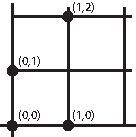
\includegraphics[width=0.25\textwidth]{1ErdosExample.pdf}
\caption{}
\label{erdos}
\end{figure}

\noindent We can compute the distances between each of the points using Euclidean distance: \\
\begin{align*}
d((0,0),(0,1)) &= \sqrt{(0-0)^2+(1-0)^2} = 1 \\
d((0,0),(1,0)) &= \sqrt{(1-0)^2+(0-0)^2} = 1 \\
d((0,0),(1,2)) &= \sqrt{(1-0)^2+(2-0)^2} = \sqrt{5} \\
d((0,1),(1,0)) &= \sqrt{(1-0)^2+(0-1)^2} = \sqrt{2} \\
d((0,1),(1,2)) &= \sqrt{(1-0)^2+(2-1)^2} = \sqrt{2} \\
d((1,0),(1,2)) &= \sqrt{(1-1)^2+(2-0)^2} = 2 
\end{align*}

\noindent Note that we obtain the same distance for some of our computations. Therefore, the only distinct distances are $1$, $\sqrt{2}$, $\sqrt{5}$ and $2$. The upper bound on the number of distinct distances is $\binom{N}{2}$, since we are picking pairs of points and computing their distance, and this process does not depend on the order of which we choose the points. From a computer scientist perspective, we would do the following computation:

$$\binom{N}{2} = \frac{N(N-1)}{2}=\frac{1}{2}N^2 -\frac{1}{2}N \sim N^2 \text{ or } O(N^2)$$

\noindent We obtain $O(N^2)$ by fining the dominant term ($N^2$) and dropping any coefficients in front of the dominant term ($\frac{1}{2}$). \\

\noindent If we obtain values randomly, it is very unlikely that we would select two of the same points (think about how many numbers are in the real numbers). There are two important questions to ask: \\

\noindent \textbf{Question 1}: How do we find the lower bound? \\
\noindent \textbf{Question 2}: How do we maximize the repetition? \\

\noindent Let's look at another example. \\

\noindent \textbf{Example}: Suppose that $N$ is a perfect square, consider a $\sqrt{N}$-lattice pictured in Figure \ref{lattice}. 

\begin{figure}[H]
\centering
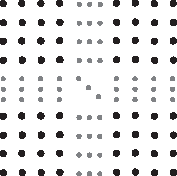
\includegraphics[width=0.35\textwidth]{1SquareLattice.pdf}
\caption{}
\label{lattice}
\end{figure}

\noindent Instead of looking for the distances, we will simplify our computations by counting the number of distinct square distances instead of regular Euclidean distance. If we construct our smallest possible squared distance is $1$ and our largest possible squared distance is $2N$. So, we can estimate that our list of distinct square distances are:
$$1, 2, \dots, 2N$$

\noindent Therefore, there is no more than $2N$ distinct squared distances. Using the same computation from the last example, we find that 
$$2N \sim N \text{ or } O(N).$$
However, this is not the best bound, because in fact, we cannot obtain 3 as a squared distance since $a^2+b^2=3$ has no solution for $a,b \in \mathbb{Z}$ (this is a result of Number Theory). Therefore, there will be holes in the list of squared distances we found. In fact, the correct lower bound of distinct distances \textit{should} be given by
$$\sim \frac{N}{\sqrt{\log(N)}} \text{ as } N \rightarrow \infty$$

\noindent In 1946, Erd\"os gave the following conjecture: \\

\noindent \textbf{Conjecture}: The number of distinct distances for $N$ is bounded below by 
$$\sim \frac{N}{\sqrt{\log(N)}} \text{ as } N \rightarrow \infty$$

\noindent The following two theorems were published in relation to this problem: \\

\noindent \textbf{Theorem} (Erd\"os 1946): The number of distinct distances for $N$ is bounded below by at least
$$\sim \sqrt{N} \text{ as } N \rightarrow \infty$$

\noindent \textbf{Theorem} (Guth, Katz 2015): The number of distinct distances for $N$ is bounded below by at least
$$\sim \frac{N}{\log(N)} \text{ as } N \rightarrow \infty$$

\noindent Another problem related to distinct distances involves \textit{crescent configurations}. We define crescent configurations to be a set of $N$ points with two properties:

\begin{enumerate}[itemsep=0pt,parsep=0pt,partopsep=0pt, topsep=0pt]
\item There exists distances $d_1, d_2, \dots, d_{N-1}$ such that distance $d_i$ appears exactly $i$ times ($1 \leq i \leq N-1$). \\
\end{enumerate}

\noindent For every $N$, we can find set of points that satisfies this property, we give the general example below in Figure \ref{linear}:

\begin{figure}[H]
\centering
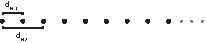
\includegraphics[width=0.6\textwidth]{1CrescentConfigurationLinear.pdf}
\caption{}
\label{linear}
\end{figure}

\noindent For this set, all of the points lie in a line and are equidistant from each other. Therefore, we additionally require the following: \\

\begin{enumerate}[itemsep=0pt,parsep=0pt,partopsep=0pt, topsep=0pt]
\addtocounter{enumi}{1}
\item The set of $N$ points must be in \textit{general position}, meaning that there is no more than two points on a line and no more than three points on a circle. \\
\end{enumerate}

\noindent These two properties define a crescent configuration.  \\


\noindent \textbf{Examples}: The existence of crescent configurations is known for up to 8 points in a set. 

\begin{figure}[H]
\centering
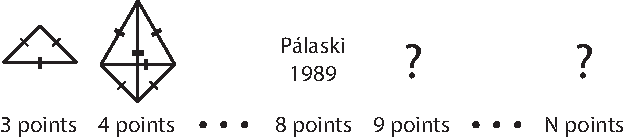
\includegraphics[width=0.75\textwidth]{1CrescentExamples.pdf}
\caption{}
\label{examples}
\end{figure}

\noindent Erd\"os conjectured that these crescent configurations cannot be geometrically realized after some $N$ for set of points in the plane. Proving the existence (or nonexistence) of a crescent configuration on $N$ points is a difficult task. In addition, we are interested in finding all possible crescent configurations for some $N$. \\

\noindent \textbf{Example}: Let $N=4$ in $\mathbb{R}^2$, Figure \ref{4points} shows all possible crescent configuration classifications that are geometrically realizable. 

\begin{figure}[H]
\centering
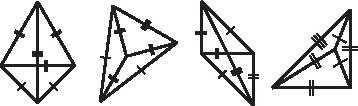
\includegraphics[width=0.75\textwidth]{1Crescent4Points.pdf}
\caption{}
\label{4points}
\end{figure}



\end{document}